\documentclass[conference]{IEEEtran}
\usepackage{amsmath,amssymb,booktabs,graphicx,multirow,tikz,balance}
\usetikzlibrary{arrows.meta,positioning,fit}
\newcommand{\method}{LockPusher}
\title{LockPusher: Object Adaptation with State-Isolated World Models for Pushing under Joint Locks}
\author{Anonymous Authors}
\begin{document}\maketitle
\begin{abstract}
Object adaptation can alter later robot forecasts through feedback in recurrent pushing models. LockPusher addresses this interaction under diagnosed joint locks by retaining a specified robot predictor while adapting object response. Analytic lock projection and separate reference and intervention rollouts preserve each branch's state and memory. The output combines reference robot forecasts with adapted object forecasts. For deterministic branches with matched initial conditions and actions, robot and pusher forecasts equal the projected reference at every step. Across 27 paired comparisons covering three historical checkpoints, three conditions, and three horizons, selective publication retains the intervention's 16.74\% mean reduction in composite object-state RMSE while preserving reference robot forecasts. Visual replanning completes all 18 core short-distance hardware trials across intact and single-joint-lock conditions.
\end{abstract}

\section{Introduction}
Model-based manipulation uses predicted object motion to select actions before execution. In contact-rich tasks such as pushing, prediction errors can change which action appears most promising \cite{finn2017visual,bauza2018data}. A joint lock further restricts the available motions. Even when the locked joint and its angle are known, the resulting object response remains uncertain. Continuing the task requires a model that incorporates the diagnosed constraint and predicts the interaction outcomes needed to choose a push.

Damage adaptation changes policies or behavior repertoires to recover task performance \cite{cully2015robots,yang2021fault}, while learned pushing models estimate contact outcomes from interaction data \cite{bauza2018data,kim2023se2}. ActivePusher connects residual physics with uncertainty-guided data acquisition and planning \cite{zhong2026activepusher}. We focus on the scope of an object update. Robot forecasts determine predicted pusher motion and can also enter action generation within candidate rollouts. In our historical coupled models, object-state error can decrease while free-state and pusher errors increase, even with zero diagnosed-lock violation (Table~\ref{tab:historical-publication}).

Enforcing a known lock and preserving the remaining robot forecast are distinct requirements. We retain a specified robot predictor while adapting the object response. In coupled recurrent models, object corrections can feed back into later robot predictions despite restricting residual outputs to object coordinates. Separate rollout states retain the object update without allowing this feedback to alter the reference prediction.

\begin{figure}[t]\centering
\includegraphics[width=\columnwidth]{figures/lockpusher_revision/task_overview.pdf}
\caption{LockPusher adapts object response under a diagnosed joint lock. The photograph shows an archived j3-lock trial. For the same candidate action, the schematic illustrates preserved robot forecasts and adapted object forecasts; it does not depict measured motion.}\label{fig:overview}
\end{figure}
LockPusher combines analytic lock projection with a state-isolated object correction. A reference predictor, called the carrier, and an intervention branch maintain separate rollout states. LockPusher returns robot coordinates from the carrier and object coordinates from the intervention branch, without feeding this combined output back into either branch. For identical initial observations and action sequences, the construction preserves the projected carrier robot trajectory at every prediction step while allowing the object forecast to change. The intervention branch retains its own robot--object dynamics, so this separation concerns the returned prediction rather than physical independence of the contact dynamics.

The adapted object forecasts rank candidate pushes by predicted terminal distance to the goal. After a portion of the selected action is executed, a fresh observation initializes the next planning cycle.

Historical paired predictions test object gains and robot preservation; a recurrence ablation tests the role of separate physical states. Hardware trials evaluate visual replanning with a robot block that satisfies preservation structurally. Initialization defects leave physical control benefits from the separate large-scale simulations unverified.

Our contributions are:
\begin{itemize}
\item A projected, state-isolated world model that permits object adaptation while preserving a specified robot forecast for matched inputs and action sequences.
\item Paired historical comparisons that separate object-prediction gains from collateral robot-prediction changes, together with a recurrence ablation of reference preservation.
\item A visual replanning implementation evaluated in intact and joint-lock hardware trials, with deployment results distinguished from the historical prediction comparisons.
\end{itemize}

\section{Related Work}
\textbf{Adaptation under changed dynamics.} Damage recovery can adapt a behavior repertoire \cite{cully2015robots}, condition a policy on inferred extrinsics \cite{kumar2021rma}, or tune simulator parameters from observations \cite{allevato2020tunenet}. These approaches change how a robot acts or how its dynamics are represented. LockPusher studies a different adaptation contract: a diagnosed joint lock is supplied, and a chosen robot predictor is retained while the object response is adapted.

\textbf{Learning pushing dynamics.} Data-efficient pushing models \cite{bauza2018data} and equivariant architectures \cite{kim2023se2} use interaction structure to improve motion prediction. Material-adaptive graph models \cite{zhang2024adaptigraph} condition dynamics on inferred physical properties. ActivePusher combines residual physics with uncertainty-guided data acquisition and kinodynamic planning \cite{zhong2026activepusher}. Our method addresses the scope of a learned correction across rollout steps. We study whether object-prediction gains can be retained while preserving a specified robot forecast. LockPusher specifies which state components may change during an adapted rollout.

\textbf{Structural priors and control.} GP pushing models support constrained MPC\cite{bauza2018data}; SE(2)-equivariant models enforce consistency under planar rigid transformations\cite{kim2023se2}; PIN-WM identifies 3D rigid-body dynamics from vision for policy transfer\cite{li2025pinwm}. These address control, geometric symmetry, and physical identification; our constraint instead concerns which predicted components may change during adaptation under a known lock.

\section{Problem Formulation}
We study planar pushing with a five-joint arm after a joint lock has been diagnosed. The observed state is $s_t=[r_t,o_t]$, with $r_t=[q_t,\dot q_t]\in\mathbb R^{10}$ and $o_t=[p_t,v_t]\in\mathbb R^4$. Here $p_t$ and $v_t$ denote planar object position and velocity. The simulation object translates with fixed orientation. An action $a_t\in\mathbb R^5$ specifies the joint command, and diagnosis $d=(m,\bar q)$ supplies a binary lock mask and the corresponding angles.

Given an observation, diagnosis, planar goal $g$, and candidate sequences $a^{(k)}_{0:H-1}$, a world model predicts terminal object positions and selects the candidate with minimum predicted distance to $g$. We require its returned robot trajectory to equal that of a specified reference predictor for the same observation and candidate. This equality defines the scope of adaptation. The reference is a design input; its preservation and accuracy are evaluated separately. Task performance is measured from executed motion.

\section{Method}
\subsection{Incorporating the diagnosed lock}
LockPusher first incorporates the known constraint into prediction. For each joint $j$, define
\begin{align}
\Pi_d(q)_j&=(1-m_j)q_j+m_j\bar q_j,\\
\Pi_d(\dot q)_j&=(1-m_j)\dot q_j,\quad
\Pi_d(a)_j=(1-m_j)a_j.
\end{align}
Object coordinates are unchanged. Applying this projection to model inputs and predicted transitions keeps locked positions fixed and locked velocities zero throughout the rollout. Because $m_j$ is binary, applying the projection twice has the same effect as applying it once. Learned object adaptation therefore operates within an explicitly constrained robot prediction.

\subsection{Object adaptation with separate rollout states}
The carrier $F_c$ supplies the reference prediction. An intervention model $F_i$ supplies the adapted object response. Each branch maintains its own physical state $s^b_t$ and recurrent state $h^b_t$, where $b\in\{c,i\}$. Starting from the same projected observation, both branches receive the same projected candidate action:
\begin{align}
(s^b_{t+1},h^b_{t+1})&=F_b(s^b_t,\Pi_d(a_t),d,h^b_t),\\
s^b_{t+1}&\leftarrow\Pi_d(s^b_{t+1}),\\
\hat s_{t+1}&=[r^c_{t+1},o^i_{t+1}].\label{eq:publish}
\end{align}
Only the returned state combines the branches. Each branch recurs on its own state, so the intervention retains its learned dynamics without changing the reference recurrence. This distinction matters when corrected object states influence later robot predictions: masking an immediate residual does not remove that later feedback path.

\textbf{Reference-trajectory preservation.} For deterministic branches with matched initial states, carrier parameters, diagnoses, and candidate actions, the returned robot trajectory equals the standalone projected carrier trajectory at every step. The initial carrier states agree. If they agree at step $t$, the same transition, hidden state, action, and projection produce the same next state. Equation~\eqref{eq:publish} returns that carrier state, establishing the result by induction. The pusher trajectory is also preserved because it is computed from joint positions by the same forward kinematics. For fixed candidates, deterministic evaluation terms computed solely from robot coordinates are also preserved. This property is relative to the chosen carrier; it establishes neither prediction accuracy nor joint dynamical consistency of the returned components.

The robot predictor is a five-node chain graph of width 136. A shared $6\!\to\!136\!\to\!136$ SiLU encoder embeds joint position, velocity, command, lock mask, lock angle, and chain depth. Two message rounds use a $272\!\to\!136\!\to\!136$ network and a 136-unit GRU; a second GRU updates temporal memory. A $136\!\to\!136\!\to\!2$ SiLU head predicts joint increments. The $140\!\to\!136\!\to\!4$ SiLU object head receives the detached mean robot code and current object state, and predicts object increments. A geometric object residual maps a 12-dimensional contact descriptor through a 16-unit Tanh hidden layer to four object corrections. The descriptor includes previous and predicted pusher positions, their displacement, pusher-to-object displacement, object velocity, and two contact gates. Each gate is $\sigma((-0.005-d)/0.002)$, where $d$ is the minimum sampled clearance in meters between two pusher capsules (radii 12 and 8 mm) and a 40-mm axis-aligned box. In this configuration, gates enter the descriptor without additionally multiplying the residual output. In the deployed configuration, the robot block does not consume object state. Separate rollout states also support the historical coupled configuration, in which publication alone must not alter either branch's recurrence.

\begin{figure*}[t]\centering
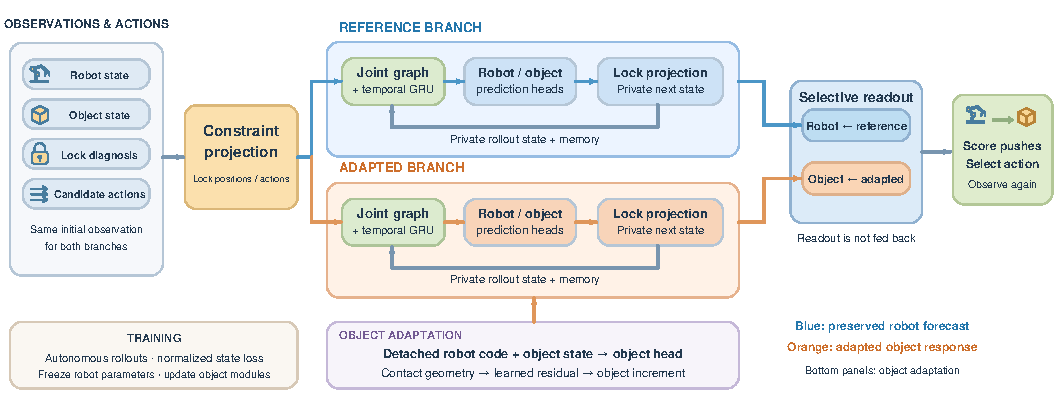
\includegraphics[width=.98\textwidth]{figures/lockpusher_revision/state_isolation.pdf}
\caption{State-isolated prediction. Both branches retain private rollout states under the same observation, actions, and diagnosed lock. Returned robot coordinates come from the reference; object coordinates come from the intervention. The deployed robot block does not receive object-state input.}\label{fig:isolation}
\end{figure*}
\subsection{Matched adaptation}
For the large-scale adaptation study, all variants start from the same pretrained carrier. We freeze its robot parameters and update the object head. LockPusher additionally updates its geometric object residual. The no-residual variant excludes this correction, while the global variant learns corrections to all state coordinates. All variants use the same data and optimization budget.

The underlying adaptation model is trained directly. Its predictions $\tilde s_t$ minimize normalized squared state errors over an autonomous prediction window; state isolation is applied when returning candidate predictions:
\begin{equation}
\mathcal L=\frac{1}{14H}\sum_{t=1}^{H}\|D^{-1}(\tilde s_t-s_t)\|_2^2.
\end{equation}
The diagonal scale matrix $D$ assigns 0.1 rad to joint positions, 1 rad/s to joint velocities, 0.03 m to object positions, and 0.1 m/s to object velocities. Frozen robot errors contribute no robot-parameter update in the object-only variants. The global residual receives supervision on robot coordinates as well. Training uses ten epochs, with five epochs at horizon 10 followed by five at horizon 25. Each trajectory supplies one randomly positioned contiguous window per epoch. Validation selects the checkpoint with minimum horizon-25 object-position MSE, including the initial checkpoint. These newly adapted weights are evaluated separately from the archived deployment weights.

\subsection{Candidate selection and execution}
For each candidate, LockPusher rolls forward and computes $\hat c_k=\|\hat p_H^{(k)}-g\|_2$. It selects $k^*=\arg\min_k\hat c_k$. A new observation reinitializes both branches after execution. Simulation executes action commands; hardware moves toward selected joint references. Their candidate construction and execution intervals are specified below.


\section{Experiments}
\label{sec:experiments}
\textbf{Simulation validity.} Initial-state audits found tool--object and tool--table penetration and joint-limit violations. Main, calibration, data-budget, and same-weight candidate comparisons therefore lack physical validation. Historical prediction uses a different, physically unchecked reset. Hardware execution is evaluated separately.

\textbf{Evaluation quantities.} Simulation endpoint error is $e_{\mathrm{goal}}=\|p_T-g\|_2$, where $p_T$ is the executed object position and $g$ the assigned goal; it is not prediction error. Goals lie 40--65 or 65--90 mm from the initial object position. All episodes, including failures, enter the mean; success is $e_{\mathrm{goal}}<30$ mm. Prediction RMSE instead compares predicted and measured coordinates. Hardware uses a separate image-space criterion: five pixels per axis for three consecutive distinct observations, with a 20-pixel core target displacement (approximately 35.1 mm). Its success rate is therefore not directly comparable to the simulation rate.

Matched contrasts with projected nominal dynamics, removal of the object residual, and global adaptation assess archived endpoint differences associated with adaptation, object correction, and correction scope. Historical publication and recurrence comparisons instead fix weights and inputs to test reference preservation.

\subsection{Simulation protocol}
The simulated arm pushes a fixed-orientation box with two translational degrees of freedom. We use five single-joint locks and four physical settings: nominal, high damping, weak motor, and mixed perturbations. High damping doubles joint damping; weak motors scale actuator gains to 70\% of nominal; the mixed setting applies both. Adaptation, validation, and testing contain 50,000, 2,000, and 6,000 independently reset trajectories, respectively, with disjoint reset seeds. Each trajectory spans 50 steps at 5 ms per step. Each variant uses six fits from the shared pretrained foundation, following the matched adaptation procedure above.

We compare LockPusher with its no-object-residual ablation, global residual adaptation, and projected nominal dynamics. Closed-loop evaluation uses 1,200 shared start--goal problems, comprising 120 problems for each lock and distance band. Each cell contains 30 problems per physical setting, with goal directions sampled uniformly within $\pm45^\circ$ of the forward axis. At each replan the controller scores 128 candidate commands over a 50-step horizon, executes ten steps, and observes the resulting state. Each episode executes five replans (0.25 s total): each predicts 0.25 s and executes 0.05 s, without stopping on goal entry. Each candidate has five ten-step constant-command segments, sampled independently from $[-0.8,0.8]$ on free joints and set to zero on the locked joint. Methods use matched problem and candidate-sampling settings, while each controller replans from its own realized state. Endpoint error is Euclidean object-to-goal distance, and success requires error below 30 mm. Position RMSE and velocity RMSE are reported separately in mm and m/s.

\subsection{Archived closed-loop comparison}
Table~\ref{tab:scale-plan} summarizes the six adaptation fits. LockPusher reduces mean endpoint error from 49.95 to 47.02 mm relative to removing the object residual. The paired improvements range from 1.79 to 5.25 mm across fits, with positive problem-bootstrap intervals in every fit (Fig.~\ref{fig:paired-plan}). Mean success rises from 24.88\% to 27.64\%. These differences hold in the archived simulator outputs; they do not establish improved physical task progress.

The mean initial goal distance is 65.07 mm; LockPusher leaves 47.02 mm, a reduction of 18.05 mm. Success requires ending within a 30 mm goal region; it does not establish precision placement. Mean net object displacement is 60.96 mm, so short execution alone cannot explain the remaining distance. ActivePusher reports mean path-wise SE(2) tracking error in Fig. 7 and uses a 100$\times$100 mm region goal\cite{zhong2026activepusher}; our terminal goal distance is not directly comparable to that mixed-pose metric.

Relative to projected nominal dynamics, LockPusher reduces mean endpoint error by 7.93 mm and increases mean success by 8.00 percentage points; paired endpoint intervals are positive in all six fits. 

Global residual adaptation achieves 45.58 mm mean endpoint error and 30.71\% success. Its endpoint error is lower than LockPusher in five of six fits; the paired intervals exclude zero in four. Thus restricting the adapted state retains the prescribed robot prediction but does not minimize endpoint error across all model classes. Open-loop position RMSE likewise does not uniformly improve after object adaptation. 

\input{sections/planning-table-en.tex}
\begin{figure*}[t]\centering
\includegraphics[width=.98\textwidth]{figures/meeting_revision/planning_three_comparisons.pdf}
\caption{Paired endpoint comparisons of LockPusher: (a) adaptation relative to projected nominal dynamics; (b) object-residual comparison relative to removing that residual; and (c) comparison with global adaptation. Positive values favor LockPusher. Each point averages 1,200 shared problems for one fit; bars are 95\% paired-problem bootstrap intervals (2,000 resamples). All panels share the same scales.}\label{fig:paired-plan}
\end{figure*}

The fixed-checkpoint prediction study is reported in the supplementary analysis, with position and velocity evaluated separately across all physical conditions. Hardware experiments use the archived deployment weights and are presented in the physical-evaluation section.

\subsection{Validation-selected residual scaling}
Candidate random draws vary with the fit seed and are shared across methods within each fit. The stratified bootstrap resamples problems within the ten lock--distance cells, carrying all methods and fits together at each sampled problem index. Intervals are conditional on these fits and their candidate draws.

A separate post-training study selects each fit's object-residual scale from $\{0,0.5,1,1.5\}$ by H50 position MSE on the existing validation set. On 2,000 fresh shared trajectories, mean per-coordinate position RMSE decreases from 21.845 to 20.750 mm. On 1,200 additional shared closed-loop problems, mean endpoint error decreases from 46.75 to 46.22 mm and success rises from 28.21\% to 28.97\%. The paired endpoint reduction is 0.532 mm, with a 95\% problem-bootstrap interval of [0.357, 0.712] mm conditional on the six fits. Three changed fits have positive intervals, one spans zero, and two retain the original scale. Relative to the no-object-residual model on these fresh problems, calibrated LockPusher reduces endpoint error by 3.398 mm (conditional 95\% interval [3.085, 3.710] mm), with positive intervals in all six fits, and raises mean success by 3.90 percentage points. This second problem set shares the initialization defect and cannot independently validate physical benefit. Global adaptation achieves 45.34 mm and 30.60\% success on these same problems. Calibration slightly reduces endpoint error, while global adaptation retains a lower mean endpoint error. The calibrated weights were not deployed on hardware.

\begin{table}[t]\centering\small
\caption{Per-fit closed-loop changes from calibration. Positive values favor calibration; intervals are conditional 95\% paired-problem bootstrap intervals.}\label{tab:calibration-fits}
\begin{tabular}{rrcr}\toprule
Fit & Scale & Error reduction (mm) & Success gain (pp)\\\midrule
7 & 1 & 0.00 [0.00, 0.00] & 0.00\\
17 & 1.5 & 1.40 [0.91, 1.91] & 1.50\\
27 & 1.5 & 0.69 [0.23, 1.16] & 1.50\\
37 & 1.5 & 0.98 [0.44, 1.56] & 2.50\\
47 & 1 & 0.00 [0.00, 0.00] & 0.00\\
57 & 1.5 & 0.11 [-0.42, 0.64] & -0.92\\
\bottomrule\end{tabular}\end{table}

\textbf{Full-state versus selective publication.} Table~\ref{tab:historical-publication} summarizes a separate historical query: checkpoints 27, 37, and 47; high damping, composition, and unseen composition; ten trajectories per condition; and horizons 10, 25, and 50. Full-state publication returns intervention robot and object coordinates; selective publication substitutes carrier robot coordinates. Both retain private branch states. Object-state errors are identical, with 16.74\% mean reduction. Full-state increases free-state RMSE in three combinations and pusher RMSE in two; selective preserves both carrier errors. Full-state improves free-state RMSE in the other 24 combinations, so preservation does not establish accuracy dominance. Object and free-state aggregates mix position with velocity. The 27 combinations reuse three checkpoints. This publication test differs from the next-state recurrence ablation below and does not establish physical control benefit.

\begin{table}[t]\centering\small
\caption{All 27 historical combinations, relative to the carrier. Object reduction averages checkpoint means. Match requires identical carrier free-state and FK-pusher squared errors in every stored window.}
\label{tab:historical-publication}
\setlength{\tabcolsep}{3pt}
\begin{tabular}{lrrrr}\toprule
& \shortstack{Object RMSE\\reduction (\%)} & \shortstack{Free\\worse} & \shortstack{Max. free\\increase (\%)} & \shortstack{Free/FK\\match}\\\midrule
Carrier & 0.00 & 0/27 & 0.00 & 27/27\\
Full-state & 16.74 & 3/27 & 6.20 & 0/27\\
Selective & 16.74 & 0/27 & 0.00 & 27/27\\
\bottomrule\end{tabular}\end{table}

\textbf{Shared-state versus isolated rollouts.} A retrospective test uses 84 previously evaluated trajectories, with 12 per physical condition. Historical weights, context, observations, and actions are fixed across the rollout alternatives. The shared-state alternative retains separate recurrent memories but feeds the combined robot--object output into both next-step transitions. The three fits and three horizons reuse these trajectories. All 63 fit--condition--horizon comparisons give identical object-position and velocity RMSE for shared-state and isolated rollouts. The isolated rollout exactly retains the standalone carrier robot prediction in every comparison; the shared-state alternative changes it in all 63. Robot diagnostic RMSE improves in 30 comparisons and worsens in 33 relative to shared-state recurrence. Isolation therefore controls reference preservation; it does not imply that the reference is more accurate. The archived closed-loop residual comparison separately reports endpoint differences after object adaptation.

\section{Real-Robot Closed-Loop Pushing}
We evaluate short-distance pushing with the five-DoF arm under intact and single-joint-lock conditions. The task requests a 20-pixel displacement along the task axis, approximately 35.1 mm under the recorded calibration. Each of the six conditions contributes three valid trials. All 18 core trials meet the criterion defined below; Table~\ref{tab:real-push} reports outcomes.

The controller uses visual object observations and joint feedback. It scores at least 10,000 candidate joint-reference sequences over a 50-step horizon, moves toward the selected reference at a 5-degree/s limit, and observes again before replanning. Figure~\ref{fig:hardware-sequence} illustrates recorded execution, while Fig.~\ref{fig:real-scene} shows the platforms.

The start gate allows two pixels per image axis. Success requires an object-to-goal error within five pixels on each axis for three distinct consecutive observed frames. The archived endpoint statistic instead uses the coordinate-wise median of the last ten detected observations. Success is determined from the consecutive frames, not this median. Within each core condition, three repetitions reuse one preparation candidate archive, transformed online using the current joint state and remaining error. Archives differ across conditions.

\begin{table}[t]\centering
\caption{Recorded closed-loop pushing outcomes. Double-lock runs use a
shorter displacement and include configuration changes; they are diagnostic
cases rather than repetitions of one fixed controller.}
\label{tab:real-push}
\begin{tabular}{lrrrr}\toprule
Condition & Goal (px) & Successes & Valid trials & Cycles\\\midrule
Intact &20&3&3&4\\
J1 lock &20&3&3&4--5\\
J2 lock &20&3&3&17\\
J3 lock &20&3&3&16--18\\
J4 lock &20&3&3&7\\
J5 lock &20&3&3&6--7\\\midrule
J1+J2 &15&1&1&14\\
J2+J3 &15&1&1&34\\
J3+J4 &15&1&3&5--31\\\bottomrule
\end{tabular}
\end{table}

Hardware candidates specify joint references $q^{\mathrm{ref}}_t$. During prediction, a PD rule generates model actions as $a_t=\Pi_d(\operatorname{clip}(5(q^{\mathrm{ref}}_t-\hat q_t)-0.5\hat{\dot q}_t,-1,1))$, using the returned robot state. Thus hardware candidate scoring includes state feedback within the rollout. With matched initial states and recurrent memories and deterministic branches, reference preservation also holds for matched reference sequences under this robot-state feedback rule: equal reference robot states produce equal actions at each step. The deployed robot block is independent of object state, so the same references yield identical robot predictions under shared-state and isolated recurrence.

Candidate references are joint offsets scaled by the remaining task-axis error, with locked references fixed at the diagnosed angles. Each observation initializes object position from the calibrated image measurement and object velocity to zero. The controller moves toward reference index 24, then observes again; it does not execute the preceding reference points. The archived strict simulation uses open-loop candidate execution, whereas the current large-scale comparison executes ten steps before replanning. Both differ from this hardware command.

All 23 formal hardware manifests record the same model configuration and the seed-27 selective checkpoint from \texttt{icra\_confirmation\_d3\_query\_selective\_w10}. Its tensors match the seed-27 residual-training checkpoint used in the archived strict simulation. These are the archived deployment weights, distinct from the newly adapted fits.

Five valid double-lock trials request a shorter 15-pixel displacement, approximately 26.3 mm. J1+J2 and J2+J3 each succeed once; J3+J4 has two failures and one success. Candidate and controller settings changed across these diagnostic cases, so they are reported individually rather than pooled as fixed-controller repetitions. Failed, invalid, and aborted attempts remain in the inventory. No matched hardware baseline was collected. The physical trials demonstrate execution, without establishing the physical validity of the archived simulation comparisons.

\begin{figure*}[t]\centering

\includegraphics[width=.98\textwidth]{figures/lockpusher_revision/hardware_sequence.pdf}
\caption{J3-lock hardware execution. Overhead frames correspond to the initial observation, half the requested task-axis displacement, and the first three-frame goal streak. Each uses the latest camera capture preceding the monitor event. Insets show the recorded start coordinate (blue) and goal tolerance (orange). The wrist view shows the initial configuration.}\label{fig:hardware-sequence}
\end{figure*}
\begin{figure*}[t]\centering

\includegraphics[width=.98\textwidth]{figures/lockpusher_revision/environment_plate.pdf}
\caption{Physical platform and CAD illustration. (a) Full-arm CAD rendering at an archived preparation configuration. (b,c) Wrist and overhead views from an archived J3 trial at different times. Quantitative simulations use a separate mechanism model with different geometry; the CAD panel illustrates the hardware configuration.}\label{fig:real-scene}
\end{figure*}

The archive also contains a same-weight candidate comparison: on 120 fresh D3 problems with 128 candidates and a 50-step open-loop execution, the deployed seed-27 checkpoint reduces terminal error by 8.72 mm relative to projected nominal dynamics (paired-problem 95\% interval [6.48, 11.04] mm). Across seeds 7, 17, and 27, reductions relative to matched carriers are 2.42, 1.65, and 0.27 mm; only seed 7 has a positive interval. This comparison shares the suspect initialization and cannot establish physical benefit for the deployed weights.

\section{Limitations and Conclusion}
LockPusher limits the scope of object adaptation under diagnosed joint locks. Separate rollout states retain the intervention's object prediction while preserving the specified robot forecast. Historical paired tests retain object-state error reductions without the observed collateral increases in carrier-relative robot error. Hardware trials demonstrate visual replanning with a configuration that satisfies preservation structurally; they do not isolate the benefit of separate rollouts. Simulation initialization defects leave physical control gains unverified.

The current evidence covers a fixed-orientation simulated box and short-distance physical pushing on one arm. Correct diagnosis is an input assumption, and preserving the carrier does not establish its accuracy. Extending this formulation to rotating objects and tasks that require adapting robot contact dynamics is a direction for further study.

\section*{Acknowledgments}
OpenAI Codex assisted with drafting and revising the abstract, introduction, related work, method, experiments, conclusion, and appendices; Chinese translation; figure and table code; and organization of the supplied experimental records.



\appendices
\section{Fixed-Checkpoint Prediction Analysis}
These historical checkpoints differ from the newly adapted closed-loop models. For seed 47 under weak motors at horizon 50, position RMSE rises from 8.63 to 28.20 mm while velocity RMSE falls from 0.152 to 0.073 m/s. A mixed-unit aggregate obscures this component tradeoff.

The fixed-checkpoint study uses 8,400 independently reset trajectories under D3 locking, with 1,200 trajectories in each of seven physical conditions and a fixed-side contact-neighborhood policy. Three existing checkpoints are evaluated at horizons 10, 25, and 50. Across all 63 checkpoint--condition--horizon combinations, the selective wrapper changes no robot coordinates relative to its carrier, and maximum diagnosed-lock violation is zero. This tests the implementation of state isolation over extended rollouts.

Figure~\ref{fig:prediction-conditions} separates object position and velocity. The historical composite metric decreases in all 27 prespecified combinations for high damping, composition, and unseen composition, averaging 16.27\%, but mixes position and velocity units. 

\subsection{Adaptation data budget}
\input{sections/data-budget-table-en.tex}
We vary the number of adaptation training trajectories while holding the number of optimization updates fixed. Nested subsets balanced across locked joints and physical profiles contain 1,000, 5,000, or 50,000 training trajectories, plus 400 validation trajectories at each budget. Three fits per method reuse the seed-27 source model's trained robot and object dynamics; the added residual heads are initialized anew. Each receives 980 updates of batch size 512, using horizons 10 and 25 for 490 updates each. For each fit, we select the checkpoint with the lowest validation H25 object-position MSE, then evaluate it on 1,200 new shared problems under the same closed-loop protocol. These counts exclude all prior source-model training and development data.

Table~\ref{tab:data-budget} reports all fits. Averaged equally over the two lower budgets, LockPusher reduces endpoint error by 3.23 mm relative to removing its object residual. All six fit--budget contrasts improve, with paired 95\% problem-bootstrap intervals excluding zero (2,000 resamples within the 40 lock--distance--profile strata, conditional on each fit). At 50,000 trajectories, two fits improve and one worsens. LockPusher's mean endpoint error does not decrease monotonically with the training budget, and global adaptation has lower mean endpoint error at each budget. These archived fits show lower endpoint error at the two lower budgets, without a monotonic scaling trend; physical benefit remains unverified.

\begin{figure*}[t]\centering
\includegraphics[width=.98\textwidth]{figures/meeting_revision/historical_absolute.pdf}
\caption{All 63 historical-model comparisons. Values are carrier RMSE minus adapted RMSE: positive means improvement, negative means degradation. Position (mm) and velocity (mm/s) use separate color scales. Seeds 27, 37, and 47 identify historical fits, not training epochs. Stars mark the historical prespecified conditions.}\label{fig:prediction-conditions}
\end{figure*}


\input{sections/appendix-method-en.tex}
\input{sections/historical-evidence-en.tex}


\bibliographystyle{IEEEtran}
\bibliography{references}
\end{document}
